\documentclass[10pt, a4paper]{article}

\usepackage{report}
\usepackage{pdfpages}

\begin{document}

\maketitle

The primary goal of this study is to assess the impact of an artificial stimulant on heart rate, considering the influence of body mass index (BMI) on this effect.
We aim to:
\begin{itemize}[nosep]
  \item Compare the effectiveness of a linear model versus a Gamma Generalized Linear Model (GLM) for analyzing the data.
  \item Estimate the treatment effect of the stimulant versus placebo on heart rate, adjusting for BMI.
\end{itemize}

\section{Preliminary Data Analysis}

The dataset contains the following variables:
\begin{itemize}[nosep]
  \item \verb|rest_pulse|: Resting heart rate (beats per minute), as recorded on the first day of the study.
  \item \verb|stimulated_pulse| Stimulated heart rate (beats per minute), as recorded on the second day of the study (after the treatment/placebo was administered).
  \item \verb|bmi|: Body Mass Index (kg/m$^2$).
  \item \verb|treatment|: Indicator for the treatment group (0 = stimulant, 1 = placebo).
\end{itemize}

\begin{figure}[ht]
  \centering
  \begin{minipage}{0.65\textwidth}
    \centering
    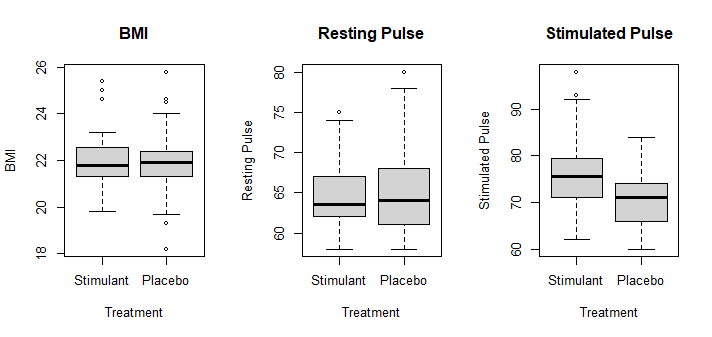
\includegraphics[width=\linewidth]{plots/data_boxplots.png}
    \caption{Data Boxplots}
    \label{fig:data_boxplots}
  \end{minipage}\hfill
  \begin{minipage}{0.3\textwidth}
    \centering
    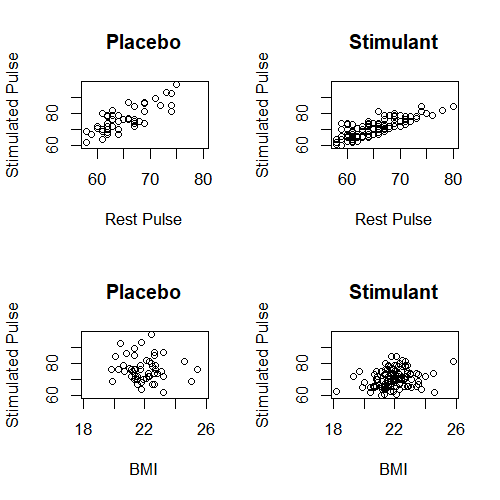
\includegraphics[width=\linewidth]{plots/data_scatter-plots.png}
    \caption{Data Scatter Plots}
    \label{fig:data_scatter-plots}
  \end{minipage}
\end{figure}

There are $118$ placebo and $56$ stimulant observations, which seems to be a reasonable sample size. But the data is not balanced, since the ratio of placebo to stimulant observations is $2.1$. A better split may be $50 \%$ for each group, which would make the data more balanced and the results more reliable.

Looking at Figure \ref{fig:data_boxplots}, we can see that the data is evenly distributed between the two treatment groups, as the boxplots for the predictors are similar in both groups. Moreover, we we can see that the stimulated pulse tends to be higher for the stimulant group compared to the placebo group. This suggests that the treatment might have an effect on the stimulated pulse, but further analysis must be conducted to confirm this.

Looking at Figure \ref{fig:data_scatter-plots}, we can see that the stimulated pulse is usually higher than the rest pulse and the relationship between them seems to be linear. This is an indication that the rest pulse might be a good predictor of the stimulated pulse. On the other hand, there is no clear relationship between the stimulated pulse and BMI. This suggests that BMI might not be a good predictor of the stimulated pulse, but further analysis must be conducted to confirm this.

\section{Models}

In order to assess the impact of the stimulant on heart rate, we fit two models:

\textbf{Linear Regression Model} (\textit{initially suggested by the clinician}): The initial model proposed involves using a linear regression framework to explain the stimulated heart rate based on the resting heart rate and treatment group. This model implicitly assumes:
\begin{itemize}
  \item \textbf{Linearity}: The relationship between the stimulated heart rate and both the resting heart rate and treatment group is linear.
  \item \textbf{Independence}: Observations (heart rates) are independent of each other.
  \item \textbf{Homoscedasticity}: The variance of the error terms is constant across all levels of the independent variables.
  \item \textbf{Normality}: The error terms are normally distributed.
\end{itemize}

This model uses the least squares method, which minimizes the sum of squared differences between observed and predicted values. By using matrix algebra, we can find the coefficients that minimize the sum of squared differences between observed and predicted values.

\textbf{Gamma Generalized Linear Model (GLM) with Inverse Link} (\textit{proposed by the data analyst}): To address the limitations of the linear model and better reflect the nature of the data, a Gamma GLM with an inverse link function was recommended. This model was chosen to account for the positive skewness observed in heart rate data and to model the difference between stimulated and resting heart rates as a function of BMI and treatment. The assumptions for this model include:
\begin{itemize}
  \item \textbf{Distribution of Response Variable}: The difference between stimulated and resting heart rates follows a Gamma distribution, which is appropriate for modeling positive continuous data with skewness.
  \item \textbf{Mean-Variance Relationship}: The variance of the response variable is a function of its mean, which is a characteristic of the Gamma distribution. This allows for more flexibility compared to the constant variance assumption in linear regression.
  \item \textbf{Independence}: Observations (heart rates) are assumed to be independent of each other.
  \item \textbf{Link Function}: The inverse link function is used to model the mean of the response variable as a function of the linear predictors. This is appropriate for modeling positive continuous data. This choice of link function is suitable for data where the effect of predictors on the response variable is multiplicative and inversely related.
\end{itemize}

In order to fit the GLM algorithm, we're going to use the Iterated Weighted Least Squares (IWLS) algorithm:
\begin{enumerate}
  \item Instead of initializing the regression coefficients (as typically done by the algorithm), we \textbf{initialize the mean} $\mu_0$ to a vector consisting of the mean of the outputs $y_i$. We do that in order to pick a good starting point for the algorithm, which is important for the convergence of the algorithm.
  \item For this model, we have the link function $\eta = \frac{1}{\mu}$, hence $\frac{\partial \eta}{\partial \mu} = -\frac{1}{\mu^2}$.
  \item \textbf{The adjusted dependent variable} ($z_i$) for weighted regression is then:
        \[
          z_i = \eta_i + (y_i - \mu_i) \left.\frac{\partial \eta}{\partial \mu}\right|_{\mu = \mu_i} = \eta_i - \frac{y_i - \mu_i}{\mu_i^2}.
        \]
  \item \textbf{The weight} ($w_i$) for weighted regression is then:
        \[
          w_{ii}^{-1} = \left(\frac{\partial \eta}{\partial \mu}\right)^2 V(\mu) = \frac{\mu^2}{\mu^4} = \frac{1}{\mu^2}
        \]
        That is because the Gamma distribution is an exponential family with canonical parameter $\theta = \frac{- \beta}{\alpha}$, dispersion parameter $\phi = \frac{1}{\alpha}$, $b(\theta) = - \log (-\theta)$, $\mu = \frac{-1}{\theta}$, and $V(\mu) = \mu^2$.
  \item \textbf{Fit the weighted regression} on the adjusted dependent variable $z_i$ with weights $w_i$.
  \item \textbf{Update the regression coefficients} ($\beta$) based on the weighted regression.
  \item \textbf{Update the linear predictor} ($\eta_i$) and \textbf{the mean}, which are given by $\eta_i = X_i \beta$ and $\mu_i = \frac{1}{\eta_i}$.
\end{enumerate}

\subsection{Linear Model}

The linear model fits quite well. By looking at the diagnostic plots (not shown), we notice that the errors have constant variance and there are no influential points in the data. But there is a slight issue with the normality of the residuals, which seem more right-skewed than a normal distribution. This suggests using a Gamma GLM with an inverse link function to better reflect the nature of the data.

We start by fitting the model \verb|pulse_diff ~ bmi + treatment, family = Gamma(link = "inverse")| and construct a $95 \%$ confidence interval for the size of the treatment effect. By using Bootstrap, we estimate the size of the treatment effect to be around $5.457723$ with a $95 \%$ confidence interval of $[4.029513, 6.923186]$.

\subsection{GLM Model Selection}

Let us try to find a better model by
\begin{lstlisting}
  Model 1: pulse_diff ~ bmi + treatment, family = Gamma(link = "inverse")
  Model 2: pulse_diff ~ bmi, family = Gamma(link = "inverse")
  Model 3: pulse_diff ~ treatment, family = Gamma(link = "inverse")
  Model 4: pulse_diff ~ bmi * treatment, family = Gamma(link = "inverse")
\end{lstlisting}
After comparing the models by looking at the deviances, the AIC, and the diagnostic plots (not shown), we've found that the best model is Model 4: this model has the lowest AIC and the lowest deviance, indicating that it may be the best model to explain the data. 

Notice that both the model proposed by the clinician and the model proposed by the statistician share the same flaw: They are unable to model the interaction between BMI and treatment. Intuitively, the pulse difference should be influenced by the BMI only for the stimulant group, and not for the placebo group. This is another reason why Model 4 is the best model: it includes this interaction.

\subsection{Best Model}

Let us analyze the best model. By looking at the diagnostic plots (not shown), we notice that the errors have constant variance, but there are a couple of influential points in the data. If we would want to, we could remove these points, but since the data is not large, we should be careful with removing observations. But in this case, we see that the errors are more normally distributed than in the linear model, which suggests that this model is an improvement over the linear model.

\begin{table}[ht]
  \centering
  \begin{tabular}{lcccc}
    \toprule
    \textbf{Coefficient} & \textbf{Estimate} & \textbf{Std. Error} & \textbf{$t$ value} & \textbf{Pr$(>|t|)$} \\
    \midrule
    (Intercept)          & 0.049042          & 0.109212            & 0.449              & 0.654               \\
    bmi                  & 0.001771          & 0.004992            & 0.355              & 0.723               \\
    treatment1           & 0.788984          & 0.165805            & 4.759              & 4.15e-06 ***        \\
    bmi:treatment1       & -0.031821         & 0.007466            & -4.262             & 3.35e-05 ***        \\
    \bottomrule
  \end{tabular}
  \caption{GLM Coefficients}
  \label{tab:glm-coefficients}
\end{table}

Looking at Table \ref{tab:glm-coefficients}, we can see that \verb|treatment1| and \verb|bmi:treatment1| are the only statistically significant coefficients. This suggests that the treatment has a significant effect on the stimulated pulse, and that the BMI has a significant effect on the stimulated pulse only for the stimulant group, which aligns with our intuition.

The significance of the coefficient \verb|bmi:treatment1| indicates that the BMI might indeed have an effect on the stimulated pulse in the treatment group, making it a good predictor for the stimulated pulse in the case of administered treatment.

\begin{table}[ht]
  \centering
  \begin{tabular}{@{}lcc@{}}
    \toprule
    \textbf{Coefficient} & \textbf{Estimate} & \textbf{95\% Confidence Interval} \\
    \midrule
    (Intercept)          & 0.049             & [-0.169, 0.257]                   \\
    bmi                  & 0.002             & [-0.008, 0.012]                   \\
    treatment1           & 0.789             & [0.457, 1.106]                    \\
    bmi:treatment1       & -0.032            & [-0.046, -0.017]                  \\
    \bottomrule
  \end{tabular}
  \caption{95\% Confidence Intervals for the coefficients}
  \label{tab:glm-confidence-intervals}
\end{table}

The confidence intervals for the coefficients are shown in Table \ref{tab:glm-confidence-intervals}. They were built using the \verb|confit()| function in R, which in this case of a Gamma GLM with an inverse link function, uses the profile likelihood method to construct the confidence intervals. This approach evaluates the likelihood of the parameter estimates across a range of values, identifying the interval within which the likelihood of the estimates does not decrease significantly from its maximum value. This method does not rely on the normal approximation, making it more accurate for distributions like Gamma, especially with non-linear link functions such as the inverse link.

\begin{figure}[ht]
  \centering
  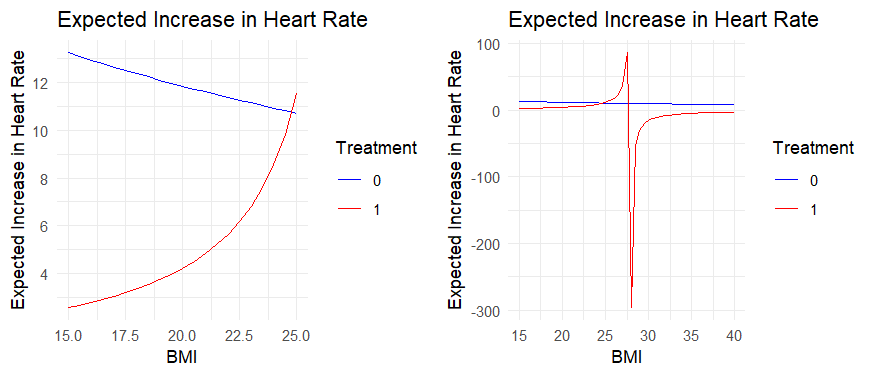
\includegraphics[width=0.6\textwidth]{plots/expected-increase-heart-rate.png}
  \caption{Expected Increase in Heart Rate}
  \label{fig:expected-increase-heart-rate}
\end{figure}

Figure \ref{fig:expected-increase-heart-rate} shows the expected increase in heart rate by varying the BMI for both groups.
\\
In the first plot, we supply the model with a range of BMI values similar to the one in the observed data, and we can see that the expected increase in heart rate is higher for the stimulant group compared to the placebo group for the most common values (that is, if we're not including the outliers, which can be seen in Figure \ref{fig:data_boxplots}). This suggests that, in the given BMI range, the stimulant has a significant effect on the stimulated pulse.
\\
In the second plot, we supply the model with a larger range of BMI values which are not present in the observed data, and we can see something interesting happening: the predictions for the pulse difference explode as the BMI increases. The trend is caused by the inverse link function being supplied with values close to $0$, resulting in an explosion of the predictions. This suggests that the model is not reliable for larger BMI values outside the range of the observed data, so more data should be collected for these values.

\begin{figure}[ht]
  \centering
  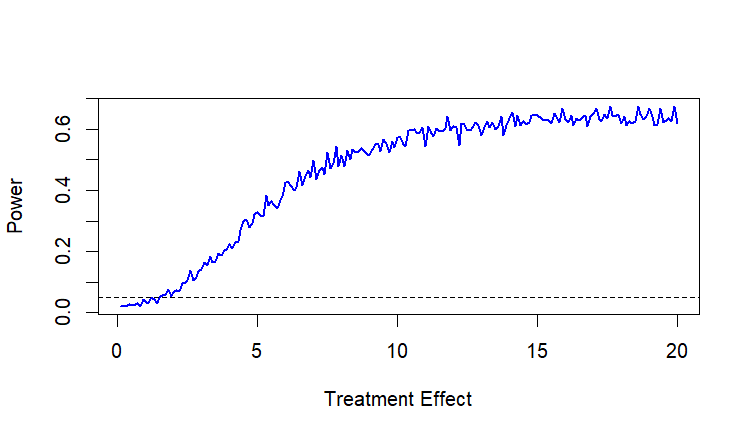
\includegraphics[width=0.4\textwidth]{plots/power.png}
  \caption{Power for different treatment effects}
  \label{fig:power}
\end{figure}

Figure \ref{fig:power} shows the power of different sizes of treatment effect. We see that, as the treatment effect increases, the power of the test increases as well. This makes sense: the larger the treatment effect, the easier it is to detect it. After around $1.6$, the power is over $0.05$, which means that from that point onwards, there are chances of detecting the treatment effect. The standard threshold for adequate power is $0.8$, which seems to not be achieved by any treatment effect from the range $[0.1, 20]$. But if we consider $0.6$ as an adequate power, then the treatment effect can be reliabily detected if its value is larger than $10.9$.

\section{Conclusion}

Here are some important conclusions from this analysis:

\begin{itemize}
  \item The data is not balanced, since the ratio of placebo to stimulant observations is $2.1$. In order to make the results more reliable, the data should be balanced, with $50 \%$ of the observations in each group.
  \item The GLM model does not generalize well for BMI values which are larger than the ones in the observed data, so more data should be collected for individuals with large BMI values.
  \item In the case the stimulant is administered, the BMI influences the stimulated pulse.
\end{itemize}

\section{Asymptotic approximations}

We need to check the following asymptotic approximations:
\begin{enumerate}
  \item The \textbf{MLE is asymptotically normal}, which means that for large sample sizes, the MLE is approximately normally distributed. This is important because it allows us to construct confidence intervals and perform hypothesis tests using the normal distribution as an approximation for the MLE.
  \item The \textbf{scaled deviances} \textbf{are asymptotically $\chi^2$-distributed} with degrees of freedom equal to the difference in the number of parameters between the full and reduced models.
\end{enumerate}

\begin{figure}[ht]
  \centering
  \begin{tabular}{lc}
    \toprule
    \textbf{Coefficient} & \textbf{$p$-value} \\
    \midrule
    Intercept            & 0.7410             \\
    bmi                  & 0.6945             \\
    treatment1           & 0.3199             \\
    bmi:treatment1       & 0.2775             \\
    \bottomrule
  \end{tabular}
  \caption{Kolmogorov-Smirnov test p-values for coefficients}
  \label{tab:p-values}
\end{figure}

We're going to check these assumptions by running a simulation study, with $1000$ iterations.

\begin{figure}[ht]
  \centering
  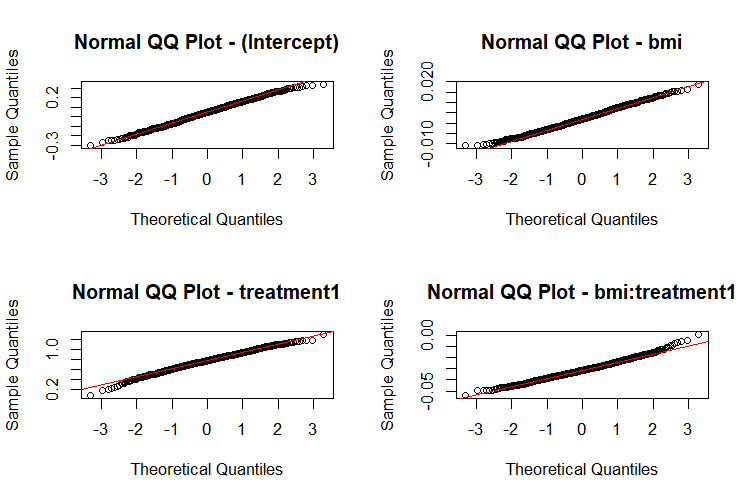
\includegraphics[width=0.6\textwidth]{plots/asymptotic_coeffs.png}
  \caption{QQ plots for the coefficients}
  \label{fig:asymptotic_params}
\end{figure}

By looking at Figure \ref{fig:asymptotic_params}, we can see that the coefficients are approximately normally distributed, which suggests that the MLE is asymptotically normal. Moreover, by looking at Table \ref{tab:p-values}, we can see that the p-values for the Kolmogorov-Smirnov test are all larger than $0.05$, which suggests that the coefficients are normally distributed.
\\
Let's also try a multivariate normal test from the \verb|MVN| package in R. We're going to use the Mardia test. The $p$-value of the Mardia skewness test is approximately $6.54-30$, while the $p$-value of the Mardia kurtosis test is approximately $0.00011$. Both of these values are smaller than $0.05$, which suggests that the data is not multivariate normal. Further analysis should be conducted to confirm this, and, in the case of non-normality, to find the cause of it.

\begin{figure}[ht]
  \centering
  \begin{minipage}{0.48\textwidth}
    \centering
    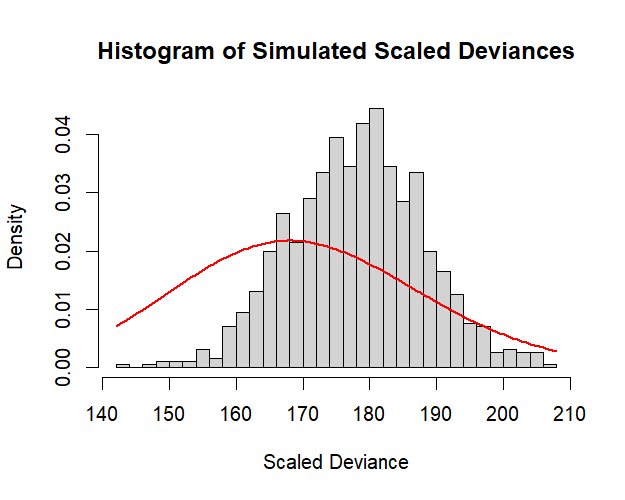
\includegraphics[width=0.65\textwidth]{plots/asymptotic_deviances_histogram.png}
    \caption{Histogram of the scaled deviances against the $\chi^2$ distribution}
    \label{fig:asymptotic_deviances_histogram}
  \end{minipage}\hfill
  \begin{minipage}{0.48\textwidth}
    \centering
    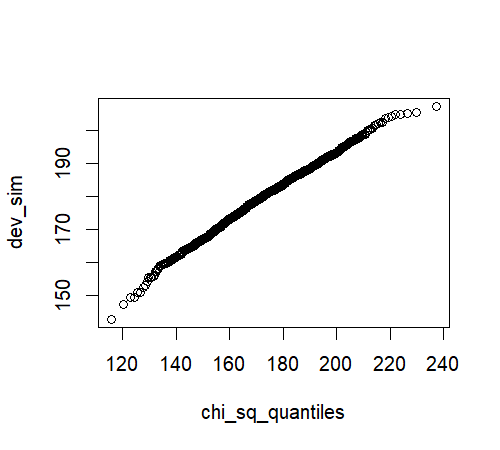
\includegraphics[width=0.65\textwidth]{plots/asymptotic_deviances_qq.png}
    \caption{QQ plot of the scaled deviances against the $\chi^2$ distribution}
    \label{fig:asymptotic_deviances_qq}
  \end{minipage}
\end{figure}

Now let's check the scaled deviances. By looking at Figure \ref{fig:asymptotic_deviances_histogram} and Figure \ref{fig:asymptotic_deviances_qq}, we can see that the scaled deviances don't seem to be $\chi^2$-distributed. They seem to be off by a translation and a scaling factor. Further analysis should be conducted to confirm this, and, in the case of non-$\chi^2$-distribution, to find the cause of it. 

Although the non-$\chi^2$-distribution of the scaled deviances can be noticed from the plots, we conduct a Kolmogorov-Smirnov test to confirm this. The $p$-value of the test is smaller than $2.2e-16$, which suggests that the scaled deviances are not $\chi^2$-distributed.

\section{Comparison with another study}

Let us start by analyzing our data.

\begin{figure}[ht]
  \centering
  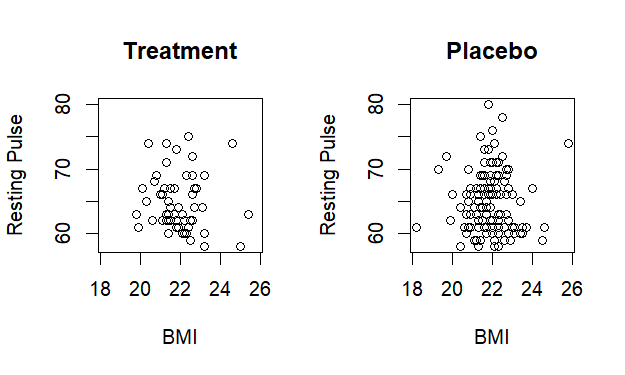
\includegraphics[width=0.5\textwidth]{plots/bmi-vs-resting-pulse_scatter-plot.png}
  \caption{Resting Pulse vs BMI}
  \label{fig:bmi-vs-resting-pulse_scatter-plot}
\end{figure}

Figure \ref{fig:bmi-vs-resting-pulse_scatter-plot} shows no sign of a clear relationship between BMI and resting pulse rate. Next, we compute the Pearson correlation coefficient between the two variables, which is $-0.028$. This indicates a very weak negative linear relationship between the two variables, but is likely not practically significant.

Overall, there seems to be no clear relationship between the two variable, whici suggests that BMI might not be a good predictor for the resting pulse.

Not let's us compare our results with the results of another study:
\\
\href{https://bmccardiovascdisord.biomedcentral.com/articles/10.1186/s12872-019-01286-2}{https://bmccardiovascdisord.biomedcentral.com/articles/10.1186/s12872-019-01286-2}

This study investigates the interaction between body mass index (BMI), exercise capacity, and the variance in resting heart rate ($\Delta$RHR) over time. It emphasizes BMI and exercise capacity as significant predictors of $\Delta$RHR, proposing that these factors could help identify individuals at increased cardiovascular risk efficiently and cost-effectively.

Findings indicate that a higher BMI and reduced exercise capacity are linked to an uptick in resting heart rate, suggesting the need for lifestyle modifications or preventive strategies to mitigate cardiovascular risk.

This contradicts the previous analysis of our data, which suggested that BMI might not be a good predictor for the resting pulse. One of the causes for this discrepancy might be the difference in the sample size: the study has a sample size of over $n = 6000$, while our sample size is $n = 174$. This suggests that the results of the study might be more reliable than the results of our analysis.

\appendix
\section{Appendix: Data Review}

After reviewing the data, we have found the following issues:

\begin{itemize}
  \item In order to get more reliable results, the data should be balanced, with $50 \%$ of the observations in each group. Our current ratio of placebo to stimulant observations is $2.1$, which clearly does not respect this condition.
  \item Our model fits well for BMI values which are similar to the ones in the observed data, but it does not generalize well for larger BMI values. More data should be collected from individuals with large BMI values, since the stimulant is likely to have a different effect on them.
  \item In the provided data, there is a notable increase in heart rate with the stimulant, one our estimation being around $5.457723$ with a $95 \%$ confidence interval of $[4.029513, 6.923186]$.
  \item In our simulation study, we've found out that in order to be at least $60 \%$ confident in detecting the treatment effect, the treatment effect should be larger than $10.9$. This suggests that the treatment effect is not easily detectable with the current sample size, and more data should be collected in order to improve the reliability of our results.
  \item The initial model is unable to capture the interaction between the BMI and the treatment: the pulse difference should be influenced by the BMI only for the stimulant group, and not for the placebo group.
\end{itemize}

\newpage

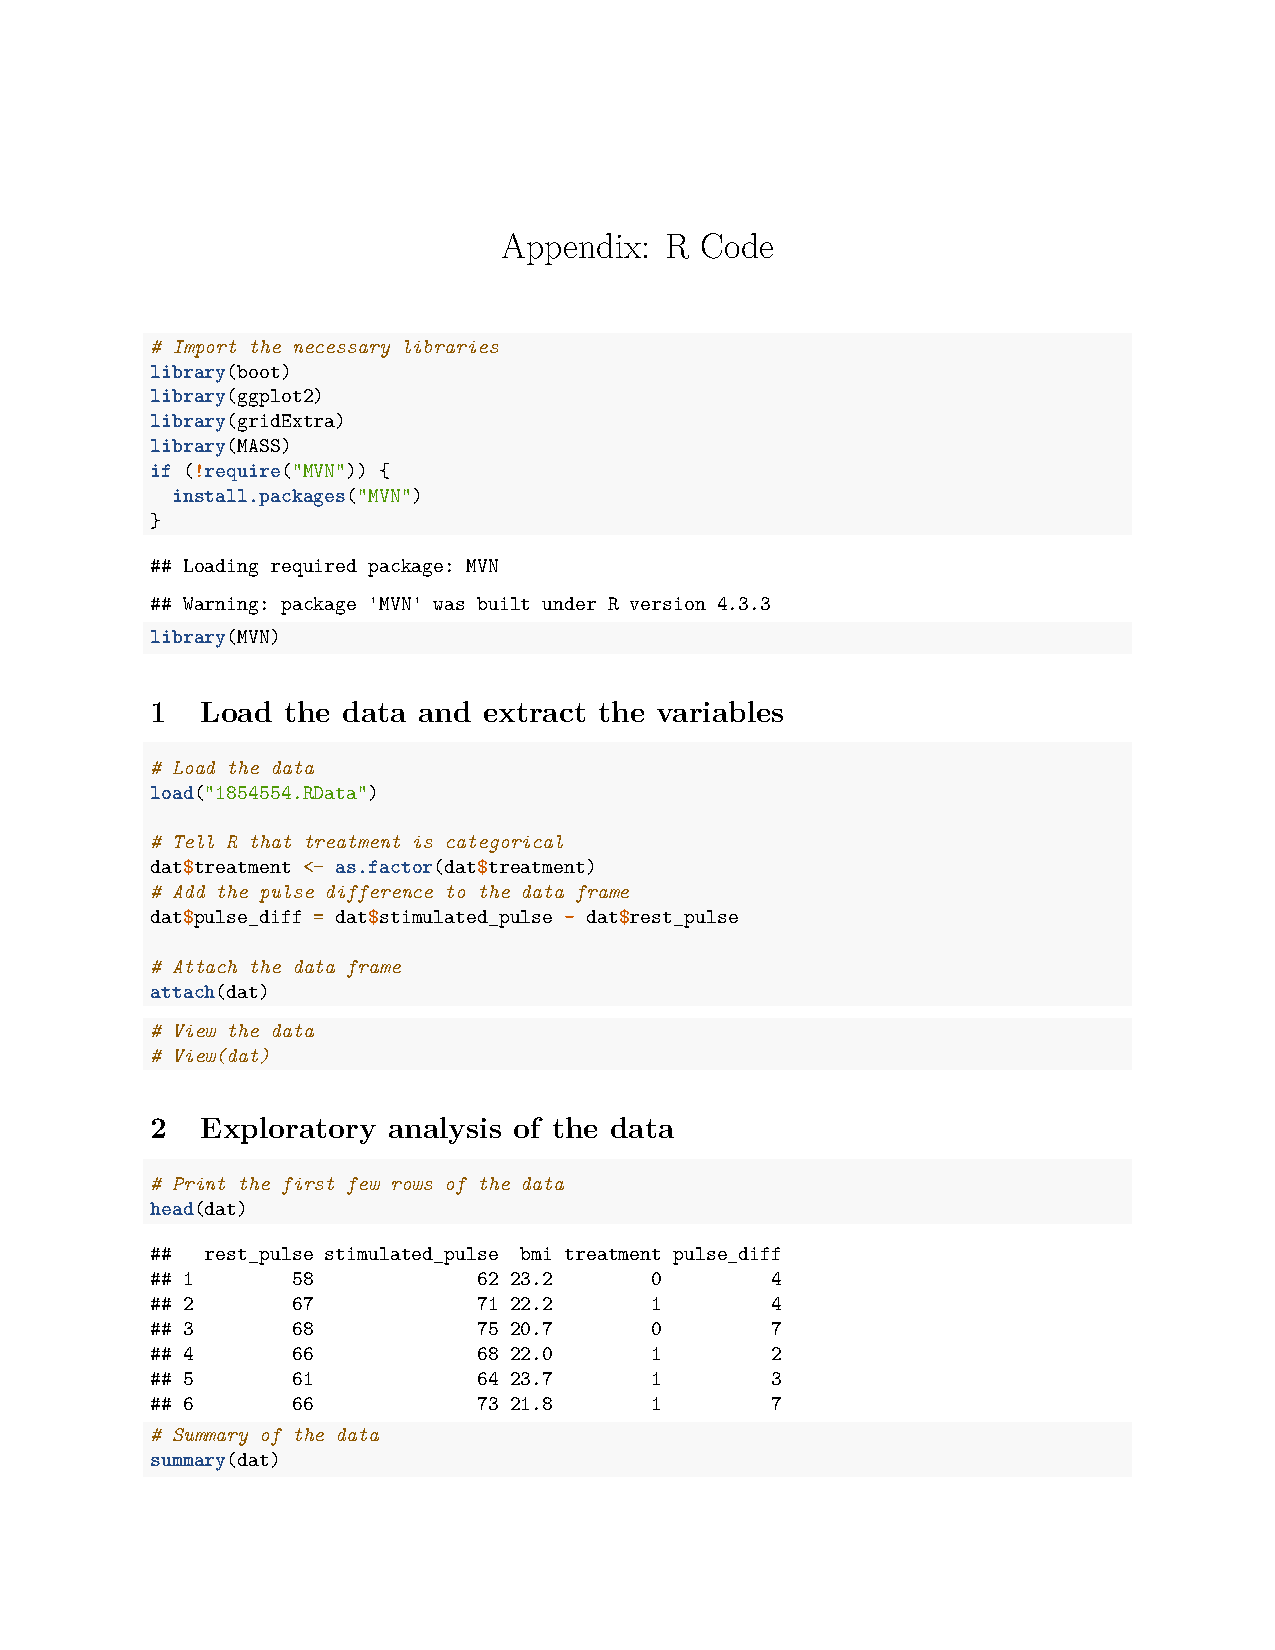
\includepdf[pages=-, pagecommand={\thispagestyle{plain}}]{implementation/code.pdf}

\end{document}